\documentclass{beamer}
\usepackage{tikz}

\usetikzlibrary{positioning}
\usetheme{Darmstadt}

\begin{document}

\title{Presentation of our Lustre-to-C compiler}
%\subtitle{}
\date{16 December 2022}
\author{Benjamin Loison, Arnaud Daby-Seesaram, Antoine Grimod}

\frame{\titlepage}

\section{Structure of the compiler}
\begin{frame}{Main ideas}
	\begin{figure}
		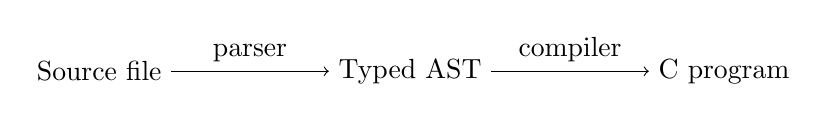
\begin{tikzpicture}
			\node (sf) {Source file};
			\node[right =2cm of sf] (ast) {Typed AST};
			\node[right =2cm of ast] (C) {C program};
			\draw
				(sf) edge[->] node[above] {parser} (ast)
				(ast) edge[->] node[above] {compiler} (C);
		\end{tikzpicture}
		\caption{Structure of the compiler}
	\end{figure}
\end{frame}

\begin{frame}{Testing}
	\begin{block}{Passes}
		The passes can be split into:
		\begin{itemize}
			\item those checking the program validity
			\item those modifying the AST of the program
		\end{itemize}
	\end{block}
\end{frame}

\section{Typed AST}
\subsection{First attempt using GADTs}
\begin{frame}
	\begin{block}{Main idea}
		Using GADTs to represent nodes and expressions allows to ensure the
		well-typedness of a program.
	\end{block}
	\begin{figure}
		\centering
		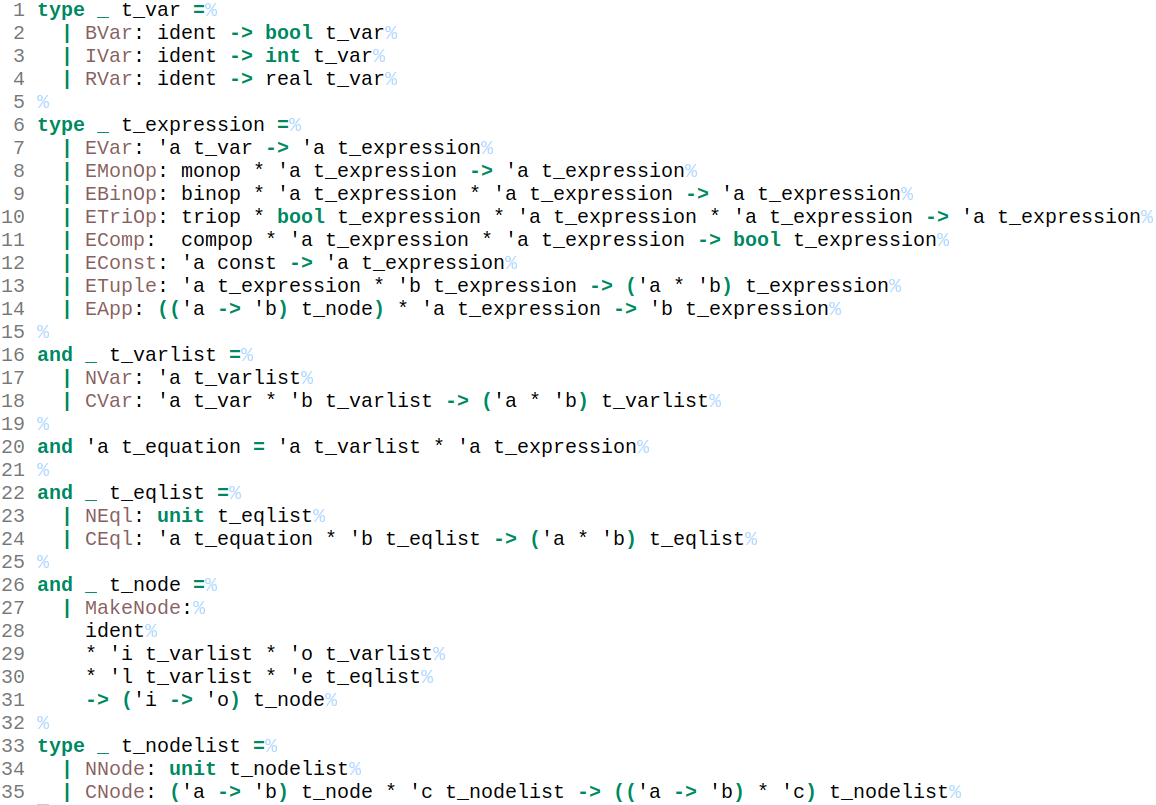
\includegraphics[width=.75\textwidth]{imgs/gadt.png}
	\end{figure}
\end{frame}
\begin{frame}
	\begin{block}{Pros of using GADTs}
		\begin{itemize}
			\item Any term of the GADT represents a well-typed program
			\item Extending the language to support more types consists of adding
				constructors to variables and constants
			\item The types are easy to read and understand
		\end{itemize}
	\end {block}

	\begin{block}{Cons of using GADTs}
		\begin{itemize}
			\item
			They cannot be dynamically generated (hence it is impossible to
			implement a parser that gives back a GADT)
			\item
			One should think about the isomorphism between
			\texttt{a $\ast$ (b $\ast$ c)} and \texttt{(a $\ast$ b) $\ast$ c}.
		\end{itemize}
	\end{block}
\end{frame}

\subsection{Second attempt: using explicit types in the variables, expressions,
\dots{} constructors}
\begin{frame}
	\begin{block}{Idea}
		Explicitly collect typing information while parsing.
	\end{block}
	\begin{figure}
		\centering
		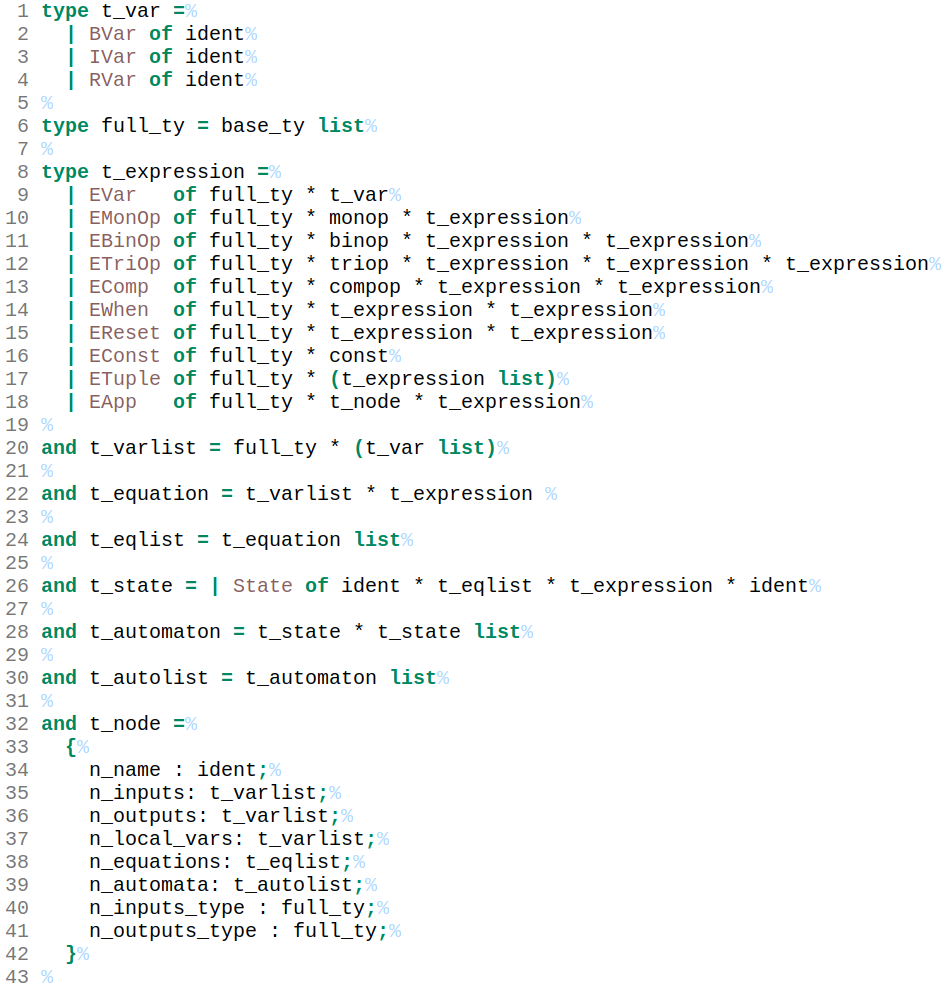
\includegraphics[width=.6\textwidth]{imgs/explicit_types.png}
	\end{figure}
\end{frame}

\begin{frame}
	\begin{block}{Pros of using explicit types}
		\begin{itemize}
			\item Programs can be built dynamically, hence a parser can be
			written
			\item While parsing, the parser has all the required information on
			the sub-variables/nodes/expressions to check the well-typedness
		\end{itemize}
	\end{block}
	\begin{block}{Cons of these definitions}
		\begin{itemize}
			\item The typing information on terms is very redundant.
			\item The rejection of ill-typed programs depends on the correctness
			of the parser
		\end{itemize}
	\end{block}
\end{frame}

\section{Passes}
\begin{frame}{Passes}
	\begin{block}{Sanity checks}
		\begin{itemize}
			\item Check the well-typedness of a program
			\item Check that there are no assignment conflicts in a programs
		\end{itemize}
	\end{block}
	\begin{block}{AST modification}
		\begin{itemize}
			\item Rewrite automata into \texttt{if-then-else} constructs
			\item Linearization of the equations
			\item (no longer required) Push the \texttt{pre} to variables
		\end{itemize}
	\end{block}
\end{frame}

\section{Translation to C}
\begin{frame}

	\texttt{ast\_to\_c.ml} architecture similar to Arnaud's AST pretty-printer.

	\pause

	For instance, go from \texttt{counting.lus} to \texttt{counting.c}.

    \pause

	Use of three tricks, as our compiler only manages \texttt{bool}s, \texttt{int}s and \texttt{float}s:
		\begin{enumerate}
			\item \texttt{0} can be interpreted as a \texttt{bool}, an \texttt{int} and a \texttt{float}
			\pause
			\item A \texttt{float} correctly encode \texttt{bool}s (\texttt{true} and \texttt{false}) and \texttt{int}s (between $[-2^{24} + 1; 2^{24} + 1]$)
			\pause
			\item To run an assignment of \texttt{value} to \texttt{variable} within the condition of a \texttt{if} and also make the cases of the \texttt{if} depends on a condition \texttt{condition}, we can do \texttt{if(((variable = value) \&\& false) || condition)}\\
			\pause
			We can also use this trick to execute an assignment and \textit{return} a value \texttt{value\_to\_return} without using any \texttt{;}, by using \texttt{((variable = value) || true) ? value\_to\_return : 0} (thanks to the first trick)
		\end{enumerate}
\end{frame}

\section{Tests}
\begin{frame}{Tests}
    \begin{block}{testing methods}
        We thought of three testing methods:
        \begin{itemize}
            \item manual testing of our functionalities
            \item run the sanity-checks-passes after any AST-altering pass
            \item simulation of the nodes (aborted)
        \end{itemize}
    \end{block}
\end{frame}

\section{Possible improvements}
\begin{frame}{Improvements}
    \begin{itemize}
        \item Increase the expressivity of the accepted programs
        \item Improve the complexity of the different passes
        \begin{itemize}
            \item Group neighbour passes of the same type (node-, expression or
            equation-pass).
        \end{itemize}
        \item \dots{}
    \end{itemize}
\end{frame}

\end{document}

